\section{Simplification}

Two functions are provided to simplify the input point set.

\ccc{CGAL::merge_simplify_point_set()} iteratively merges pairs of points which are epsilon-closed.\\
This algorithm is precise but slower than \ccc{CGAL::random_simplify_point_set()}.

\ccc{CGAL::random_simplify_point_set()} randomly deletes a user-specified fraction of points from the input point set.\\
This algorithm is very fast.

\ccRefIdfierPage{CGAL::merge_simplify_point_set}  \\
\ccRefIdfierPage{CGAL::random_simplify_point_set}  \\

% Insert image merge_simplification.jpg/eps
\begin{center}
    \label{Point_set_processing_3-fig-merge_simplification}
    % Image
    \begin{ccTexOnly}
        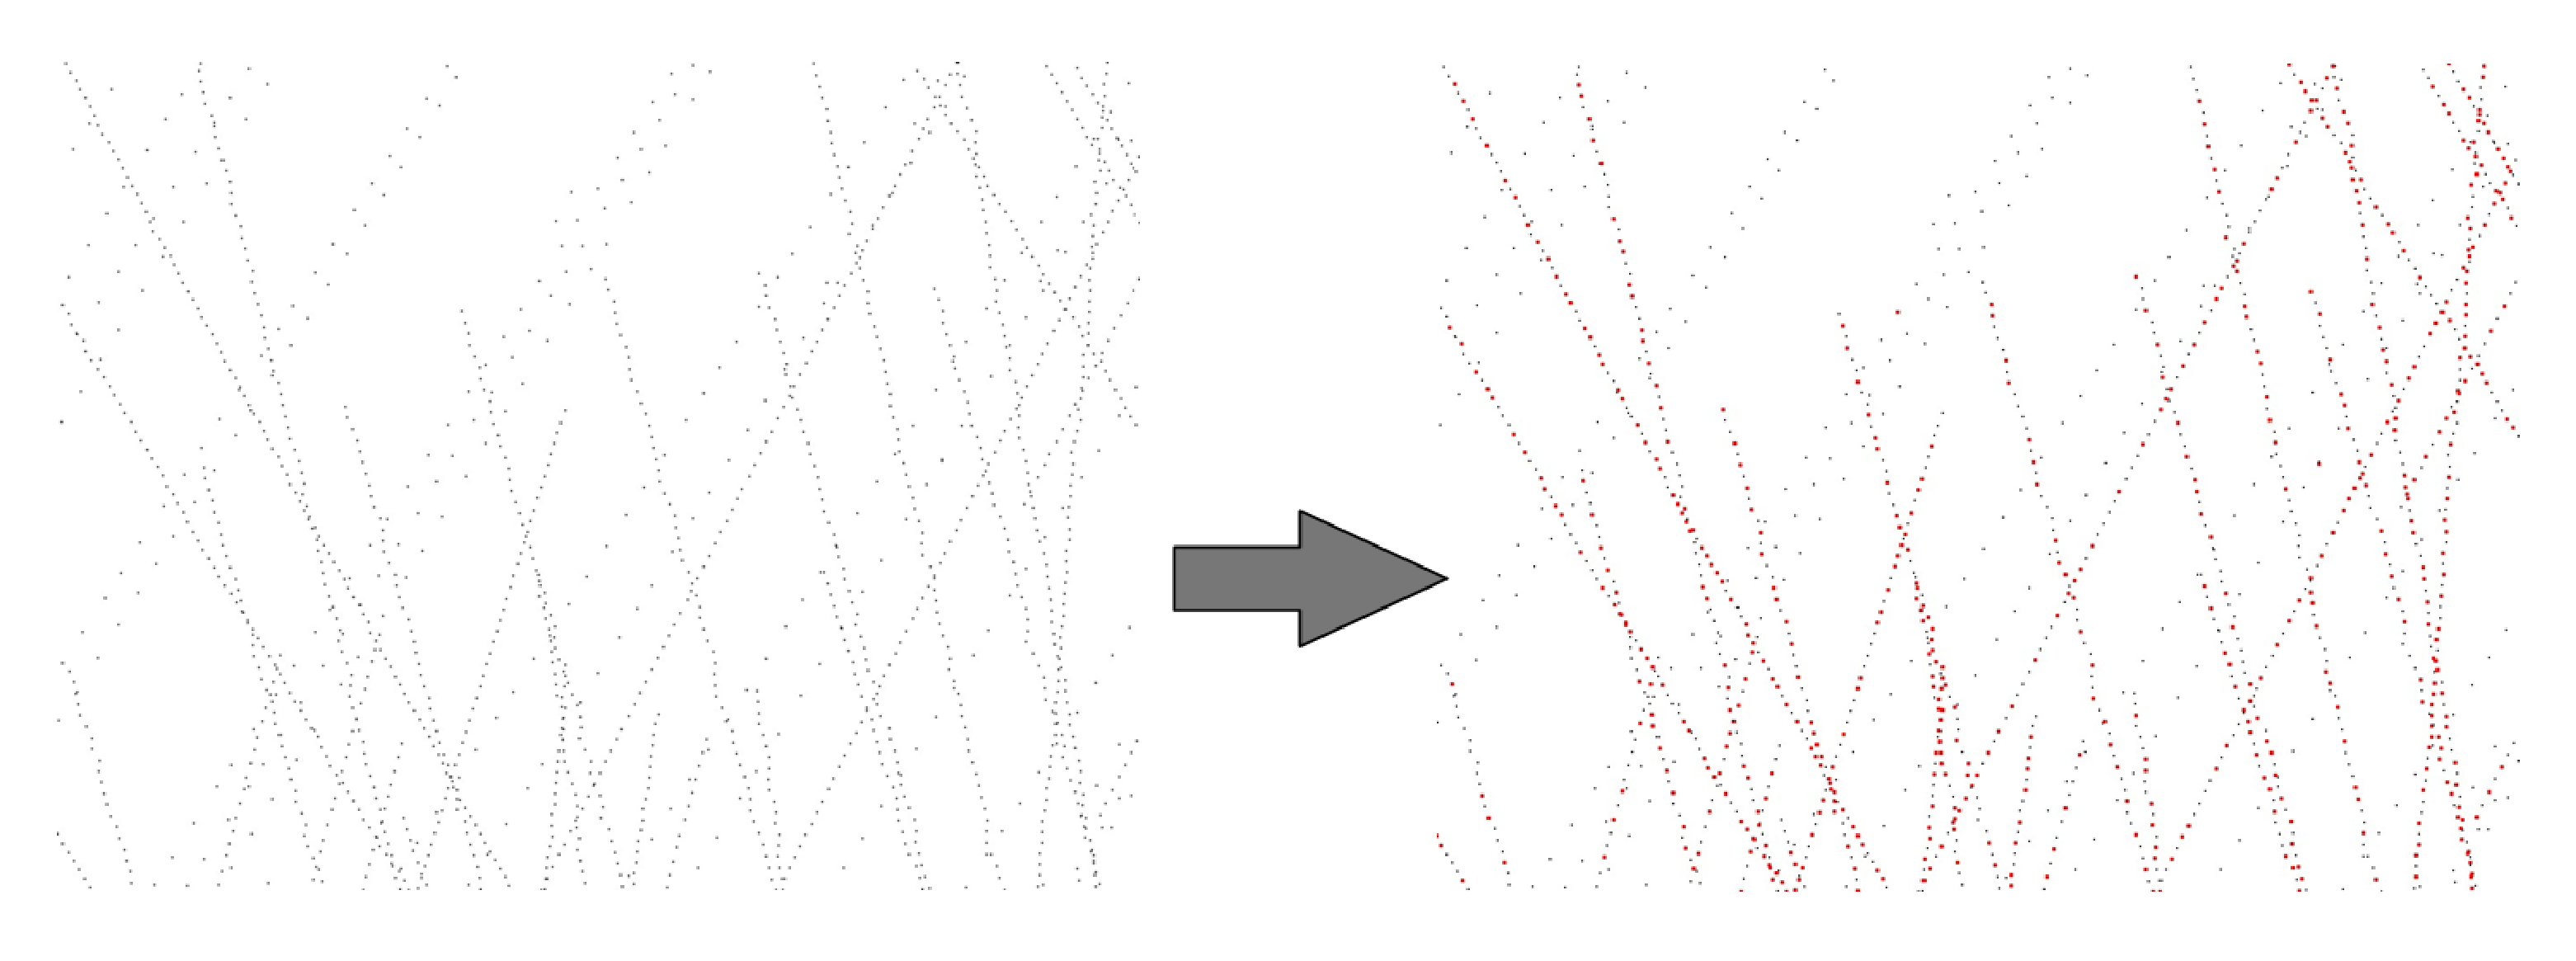
\includegraphics[width=1.0\textwidth]{Point_set_processing_3/merge_simplification} % omit .eps suffix
    \end{ccTexOnly}
    \begin{ccHtmlOnly}
        <img width="100%" border=0 src="../Point_set_processing_3/merge_simplification.jpg"><P>
    \end{ccHtmlOnly}
    % Title
    \begin{figure}[h]
        \caption{Point set simplification by merging.
                 Left: input point set.
                 Right: removed points are depicted in red.}
    \end{figure}
\end{center}

Example:

\ccIncludeExampleCode{Point_set_processing_3/random_simplification_example.cpp}